\documentclass[answers]{exam}
\renewcommand{\solutiontitle}{\noindent\textbf{}\par\noindent}

\usepackage{fullpage} % Package to use full page
\usepackage{parskip} % Package to tweak paragraph skipping
\usepackage{tikz} % Package for drawing
\usepackage{amsmath}
\usepackage{blindtext}
%\usepackage{hyperref}
\usepackage{graphicx}
\usepackage{enumerate}
\usepackage{caption}
\usepackage{subcaption}
\usepackage{multicol}
\usepackage{mathptmx}
\usepackage{amsmath}
\usepackage{amssymb}
\usepackage{nameref}
\usepackage{minted}
\usepackage{graphicx}

\newcommand{\mypoints}[1]{\textcolor{red}{(#1 points)}}
\newcommand{\achuta}[1]{\textcolor{magenta}{Achuta: #1}}
\newcommand{\chinmay}[1]{\textcolor{orange}{Chinmay: #1}}
\newcommand{\albert}[1]{\textcolor{purple}{Albert: #1}}
\newcommand{\myinput}[1]{\textcolor{blue}{#1}}

\title{\normalfont \normalsize
\textsc{{Department of Electrical and Computer Engineering, UCLA \\
EC ENGR 188: Introduction to Computer Vision}}
\date{\vspace{-12ex}}
}
\begin{document}
\maketitle
\rule{\linewidth}{0.8pt} \\[6pt] 
\noindent
\large\textbf{\textsc{Instructor:}} Prof. Achuta Kadambi, Prof. Stefano Soatto \hfill \large\textbf{\textsc{Name:}} \myinput{Anuj Agrawal}\\
\large\textbf{\textsc{TA:}} Zhen Wang \hfill 
\large\textbf{\textsc{UID:}} \myinput{605627630}
\rule{\linewidth}{0.8pt} \\[6pt] 

\begin{center}
{\textsc{Homework 1}} 
\end{center}
% \vspace{2cm}


\begin{table}[h]
\centering
\resizebox{0.8\textwidth}{!}{%
\begin{tabular}{cccc}
\hline
\multicolumn{1}{c}{\textsc{Problem}} &
\multicolumn{1}{c}{\textsc{Type}} &
\multicolumn{1}{c}{\textsc{Topic}} & \multicolumn{1}{c}{\textsc{Max. Points}} \\  \hline \\ 
 \ref{Signal Processing 101} & Analytical & LSI Systems &  10 \\ [2mm]
  2 & Coding & 2D-Convolution &  5 \\ [2mm]
  3 & Coding & Image Blurring and Denoising &  15 \\ [2mm]
 4 & Coding & Image Gradients &  5 \\ [2mm]
 5 & Analytical + Coding & Image Filtering &  15 \\  [2mm]
 6 & Analytical & Interview Question (Bonus) &  10 \\
 [2mm]
    \hline
\end{tabular}
}
\caption*{}
\label{}
\end{table}
\section*{Motivation}

The long-term goal of our field is to teach robots how to see. The pedagogy of this class (and others at peer schools) is to take a \emph{bottom-up} approach to the vision problem. To teach machines how to see, we must first learn how to represent images (lecture 2), clean images (lecture 3), and mine images for features of interest (edges are introduced in lecture 4 and will thereafter be a recurring theme). This is an evolution in turning the  matrix of pixels (an unstructured form of ``big data") into something with structure that we can manipulate.

The problem set consists of: 
\begin{itemize}
    \item analytical questions to solidify the concepts covered in the class, and
    \item coding questions to provide a basic exposure to image processing using Python.
\end{itemize}

\emph{You will explore various applications of convolution such as image blurring, denoising, filtering and edge detection. These are fundamental concepts with applications in many computer vision and machine learning applications. You will also be given a computer vision job interview question based on the lecture.}

\section*{Homework Layout}
The homework consists of 6 problems in total, with subparts for each problem. There are 2 types of problems in this homework - analytical and coding. All the problems need to be answered in the Overleaf document. Make a copy of the Overleaf project, and fill in your answers for the questions in the solution boxes provided. 

For the analytical questions you will be directly writing their answers in the space provided below the questions. For the coding problems you need to use the Jupyter notebook provided Jupyter notebook (see the Jupyter notebook for each sub-part which involves coding). After writing your code in the Jupyter notebook you need to copy paste the same code in the space provided below that question on Overleaf. For instance, for Question 2 you have to write a function `conv2D` in the Jupyter notebook (and also execute it) and then copy that function in the box provided for Question 2 here in Overleaf. In some questions you are also required to copy the saved images (from Jupyter) into the solution boxes in Overleaf. For instance, in Question 3.2 you will be visualizing the gaussian filter. So you will run the corresponding cells in Jupyter (which will save an image for you in PDF form) and then copy that image in Overleaf.

\section*{Submission}

You will need to make two submissions: (1) Gradescope: You will submit the Overleaf PDF with all the answers on Gradescope. (2) CCLE: You will submit your Jupyter notebook (.ipynb file) with all the cells executed on CCLE. 

\section*{Software Installation}

You will need Jupyter to solve the homework. 
You may find these links helpful: 
\begin{itemize}
    \item Jupyter (https://jupyter.org/install)
    \item Anaconda (https://docs.anaconda.com/anaconda/install/)
\end{itemize}

\newpage
\section{Image Processing}
\label{Signal Processing 101}
\subsection{Periodic Signals \mypoints{1.0}}
Is the 2D complex exponential $x(n_1, n_2) = \exp(j(\omega_1n_1 + \omega_2 n_2))$ periodic in space? Justify.
\begin{solution}
In continuous space, the given signal is always periodic in space with a periodicity of $2\pi/\omega_o$.
In discrete space, the given signal is periodic in space only when\\
$\omega_o N=2 \pi m$, where n, m $\in  \mathbb{Z}$,\\
$\omega_o/ 2\pi = m/n$\\
i.e. $\omega_o/ 2\pi$ is a rational number
\end{solution}

\subsection{ Working with LSI systems \mypoints{3.0}}\label{sssec:Linearity}
Consider an LSI system $T[x] = y$ where $x$ is a 3 dimensional vector, and $y$ is a scalar quantity. We define 3 basis vectors for this 3 dimensional space: $x_1 = [1,0,0]$, $x_2 = [0,1,0]$ and $x_3 = [0,0,1]$. \\
(i) Given $T[x_1] = a$, $T[x_2] = b$ and $T[x_3] = c$, find the value of $T[x_4]$ where $x_4 = [5,4,3]$. Justify your approach briefly (in less than 3 lines).\\
(ii) Assume that $T[x_3]$ is unknown. Would you still be able to solve part (i)? \\ 
(iii) $T[x_3]$ is still unknown. Instead you are given $T[x_5] = d$ where $x_5 = [1,-1,-1]$. Is it possible to now find the value of $T[x_4]$, given the values of $T[x_1], T[x_2]$ (as given in part (i)) and $T[x_5]$? If yes, find $T[x_4]$ as a function of $a,b,d$; otherwise, justify your answer.
\begin{solution}
(i) Given that the system is LSI it follows, \\
$T[\alpha_{1} x_{1} (n_1, n_2) + \alpha_{2} x_{2} (n_1, n_2)] = \alpha_{1}T[x_{1}(n_1, n_2)] + \alpha_{2}T[x_{2}(n_1, n_2)]$\\
$x_4 = [5, 4, 3]$, can be written as a linear combination of the three basis vectors s.t.\\
$x_4 = [5, 4, 3] = 5[1, 0, 0] + 4[0, 1, 0] + 3[0, 0, 1] = 5x_1 + 4x_2 + 3x_3$\\
Therefore $T[x_4] = 5T[x_1] + 4T[x_2] +3T[x_3] = 5a+4b+3c$

(ii) We won't be able to solve part (i) if $T[x_3]$ is unknown as no linear combination of basis vectors $x_1$ and $x_2$ will give $x_4$ since the z component of both these basis vectors are zero. Hence no linear combination of their respective system outputs (i.e. $T[x_1] and T[x_2]$) can solve for $T[x_4]$.

(iii) $x_4 = [5, 4, 3] = \alpha_1[1, 0, 0] +\alpha_2[0, 1, 0] + \alpha_3[1, -1, -1]$\\
Solving the above equation gives, $\alpha_1 = 4, \alpha_2= 1, \alpha_3 = -3 $\\
Therefore $T[x_4] = 4T[x_1] + 1T[x_2] -3T[x_5] = 4a+1b-3d$\\

\end{solution}

\subsection{ Space invariance \mypoints{2.0}}\label{sssec:Space_Invariance}
Evaluate whether these 2 linear systems are space invariant or not. (The answers should fit in the box.) \\
(i) $T_1[x(n_1)] = 2x(n_1)$ \\
(ii) $T_2[x(n_1)] = x(2n_1)$. 
\begin{solution}

For a LSI system, if $g(n_1) = T[x(n_1)]$ and $x_{n_o}(n_1) \triangleq x(n_1-n_0)$ then\\
$g_{n_o}(n_1) = T[x_{n_o}(n_1)] = g(n_1 - n_o)$

(i) $T_1[x(n_1)] = 2x(n_1)$ \\
For, $x_{n_o}(n_1)$, $T_1[x_{n_o}(n_1)] = 2x_{n_o}(n_1) = 2x(n_1 - n_o)$\\
Also, $g(n_1) = 2f(n_1)$, where $f(n_1) = x(n_1 - n_o)$ implies $g(n_1) = 2x(n_1 - n_o)$ \\
as $T_1[x_{n_o}(n_1)] = g(n_1)$ the system is space invariant.

(ii) $T_2[x(n_1)] = x(2n_1)$.\\
For, $x_{n_o}(n_1)$, $T_1[x_{n_o}(n_1)] = x_{n_o}(2n_1 - 2n_o)$\\
Also, $g(n_1) = f(2n_1)$, where $f(n_1) = x(n_1 - n_o)$ implies $g(n_1) = x(2n_1 - n_o)$ \\
as $T_1[x_{n_o}(n_1)] \neq g(n_1)$ the system is not space invariant.
\end{solution}


\subsection{Convolutions \mypoints{4.0}}\label{sssec:Convolutions}


\begin{figure}[h]
    \centering
    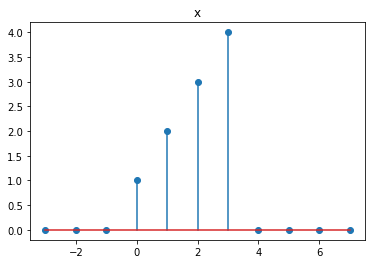
\includegraphics[width=0.3\linewidth]{Images/x.png}
    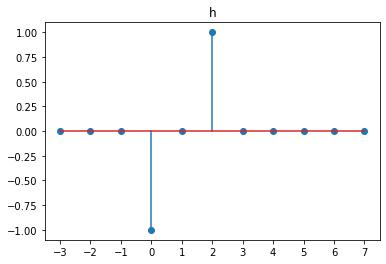
\includegraphics[width=0.31\linewidth]{Images/h.png}
    \caption{(a) Graphical representation of $x$ (b) Graphical representation of $h$}
    \label{fig:my_label}
\end{figure}
Consider 2 discrete 1-D signals $x(n)$ and $h(n)$ defined as follows:  
\begin{equation}
    \begin{aligned}
    x(i) &= i + 1 \quad \forall i \in \{0,1,2,3\} \\
    x(i) &= 0 \quad \forall i \not\in \{0,1,2,3\}\\
    h(i) &= i - 1 \quad \forall i \in \{0,1,2\} \\
    h(i) &= 0 \quad \forall i \not\in \{0,1,2\}\\
    \end{aligned}
\end{equation}
(i) Evaluate the discrete convolution $h * x$. \\
(ii) Show how you can evaluate the non-zero part of $h * x$ as a product of 2 matrices $H$ and $X$. Use the commented latex code in the solution box for typing out the matrices. 
\begin{solution}
(i) y[n] =  $h[n] * x[n]$ = $\sum_{i=-\infty}^{\infty} x[i]h[n-i]$ \\
{\small $y[n] =\{ 1(-1)], [(2(-1) + 1(0)], [3(-1) + 2(0) + 1(1)], [4(-1) + 3(0) + 2(1)], [4(0) + 3(1)], [4(1)]\}$\\}
$y[n] =\{-1, -2, -2, -2, 3, 4\}$

(ii) The given convolution of signals can bw written as a multiplication of two matrices by the Toeplitz method. 
Let,

$h[n] = [-1, 0, 1]$\\
$x[n] = [1, 2, 3, 4]$\\


then Toeplitz matrix of $x[n],$ $ D_n(x[n]) = \begin{bmatrix}
1 & 0 & 0\\
2 & 1 & 0\\
3 & 2 & 1\\
4 & 3 & 2\\
0 & 4 & 3\\
0 & 0 & 4\\
\end{bmatrix}$\\

y[n] =  $h[n] * x[n]$ = $D_n(x[n]) .  h[n]$ =$x[n]. D_n(h[n])$\\
$
\begin{bmatrix}
-1\\
-2\\
-2\\
-2\\
3\\
4\\
\end{bmatrix}
$
=
$
\begin{bmatrix}
1 & 0 & 0\\
2 & 1 & 0\\
3 & 2 & 1\\
4 & 3 & 2\\
0 & 4 & 3\\
0 & 0 & 4\\
\end{bmatrix}
$
$
\begin{bmatrix}
-1\\
0\\
1\\
\end{bmatrix} \\
$
$y[n] =\{-1, -2, -2, -2, 3, 4\}$

\end{solution}
\newpage

\section{2D-Convolution \mypoints{5.0}} 

In this question you will be performing 2D convolution in Python. Your function should be such that the convolved image will have the same size as the input image i.e. you need to perform zero padding on all the sides. 
(See the Jupyter notebook.)

\textit{This question is often asked in interviews for computer vision/machine learning jobs.}

Make sure that your code is within the bounding box below.
\begin{solution}
% \vspace{2cm} % remove this
% Paste your code within the block
\begin{minted}{python}
def conv2D(image: np.array, kernel: np.array = None):
  k_shape = kernel.shape #shape of the kernel
  pad_factor = int(k_shape[0]/2) #padding each side
  i_shape = image.shape #shape of the input image
  image = np.pad(image, ((pad_factor,pad_factor),(pad_factor,pad_factor)), 
                 'constant') #padded image
  i_new_shape = image.shape #shape of the new image
  conv_matrix = np.zeros(i_shape) #New convoluted image (all zeros)
  
  for i in range(i_new_shape[0] - k_shape[0] + 1):
    for j in range(i_new_shape[0] - k_shape[0] + 1):
      conv_matrix[i][j] = \
      np.sum(np.multiply(image[i:i+k_shape[0],j:j+k_shape[0]],kernel))
      
  return conv_matrix
\end{minted}
\end{solution}

\newpage
\section{Image Blurring and Denoising \mypoints{15.0}}
In this question you will be using your convolution function for image blurring and denoising. Blurring and denoising are often used by the filters in the social media applications like Instagram and Snapchat. 

\subsection{Gaussian Filter \mypoints{3.0}}
In this sub-part you will be writing a Python function which given a filter size and standard deviation, returns a 2D Gaussian filter. (See the Jupyter notebook.)

Make sure that your code is within the bounding box.
\begin{solution}
% \vspace{2cm} % remove this
% Paste your code within the block
\begin{minted}{python}
def gaussian_filter(size: int, sigma: float):
    kernel = np.zeros((size,size)) #empty kernel
    mx = size//2 #mean x
    my = size//2 #mean y
    c = 1 / (2*(sigma**2)*np.pi)
    for i in range(size):
        for j in range(size):
            kernel[i,j] = c*np.exp((-(i-mx)**2-(j-my)**2)/(2*(sigma**2)))
    return kernel/(np.sum(kernel))
\end{minted}
\end{solution}

\subsection{Visualizing the Gaussian filter \mypoints{1.0}}

(See the Jupyter notebook.) You should observe that increasing the standard deviation ($\sigma$) increases the radius of the Gaussian inside the filter.

Copy the saved image from the Jupyter notebook here.
\begin{solution}
% \vspace{2cm} % remove this
% Upload the image the Images folder in the project and then just un-comment the lines below.
\begin{figure}[H]
    \centering
    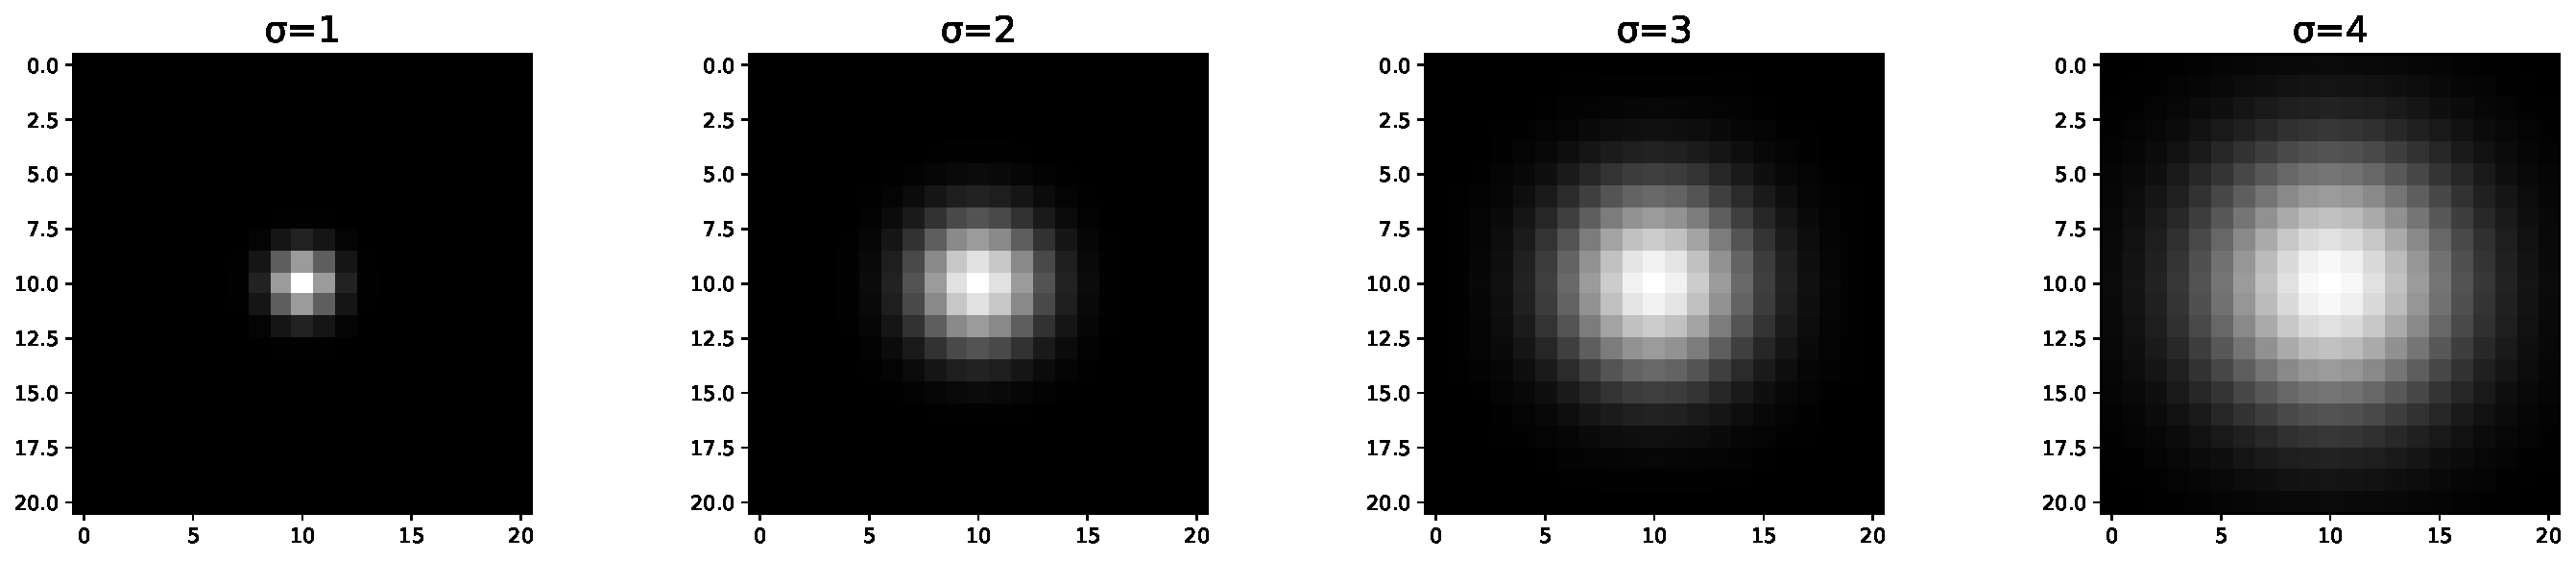
\includegraphics[width=1.0\linewidth]{Images/question_3_2.pdf}
\end{figure}
\end{solution}

\subsection{Image Blurring: Effect of increasing the filter size and $\sigma$ \mypoints{1.0}}

(See the Jupyter notebook.) You should observe that the blurring should increase with the kernel size and the standard deviation.

Copy the saved image from the Jupyter notebook here.
\begin{solution}
% \vspace{2cm} % remove this
% Upload the image the Images folder in the project and then just un-comment the lines below.
\begin{figure}[H]
    \centering
    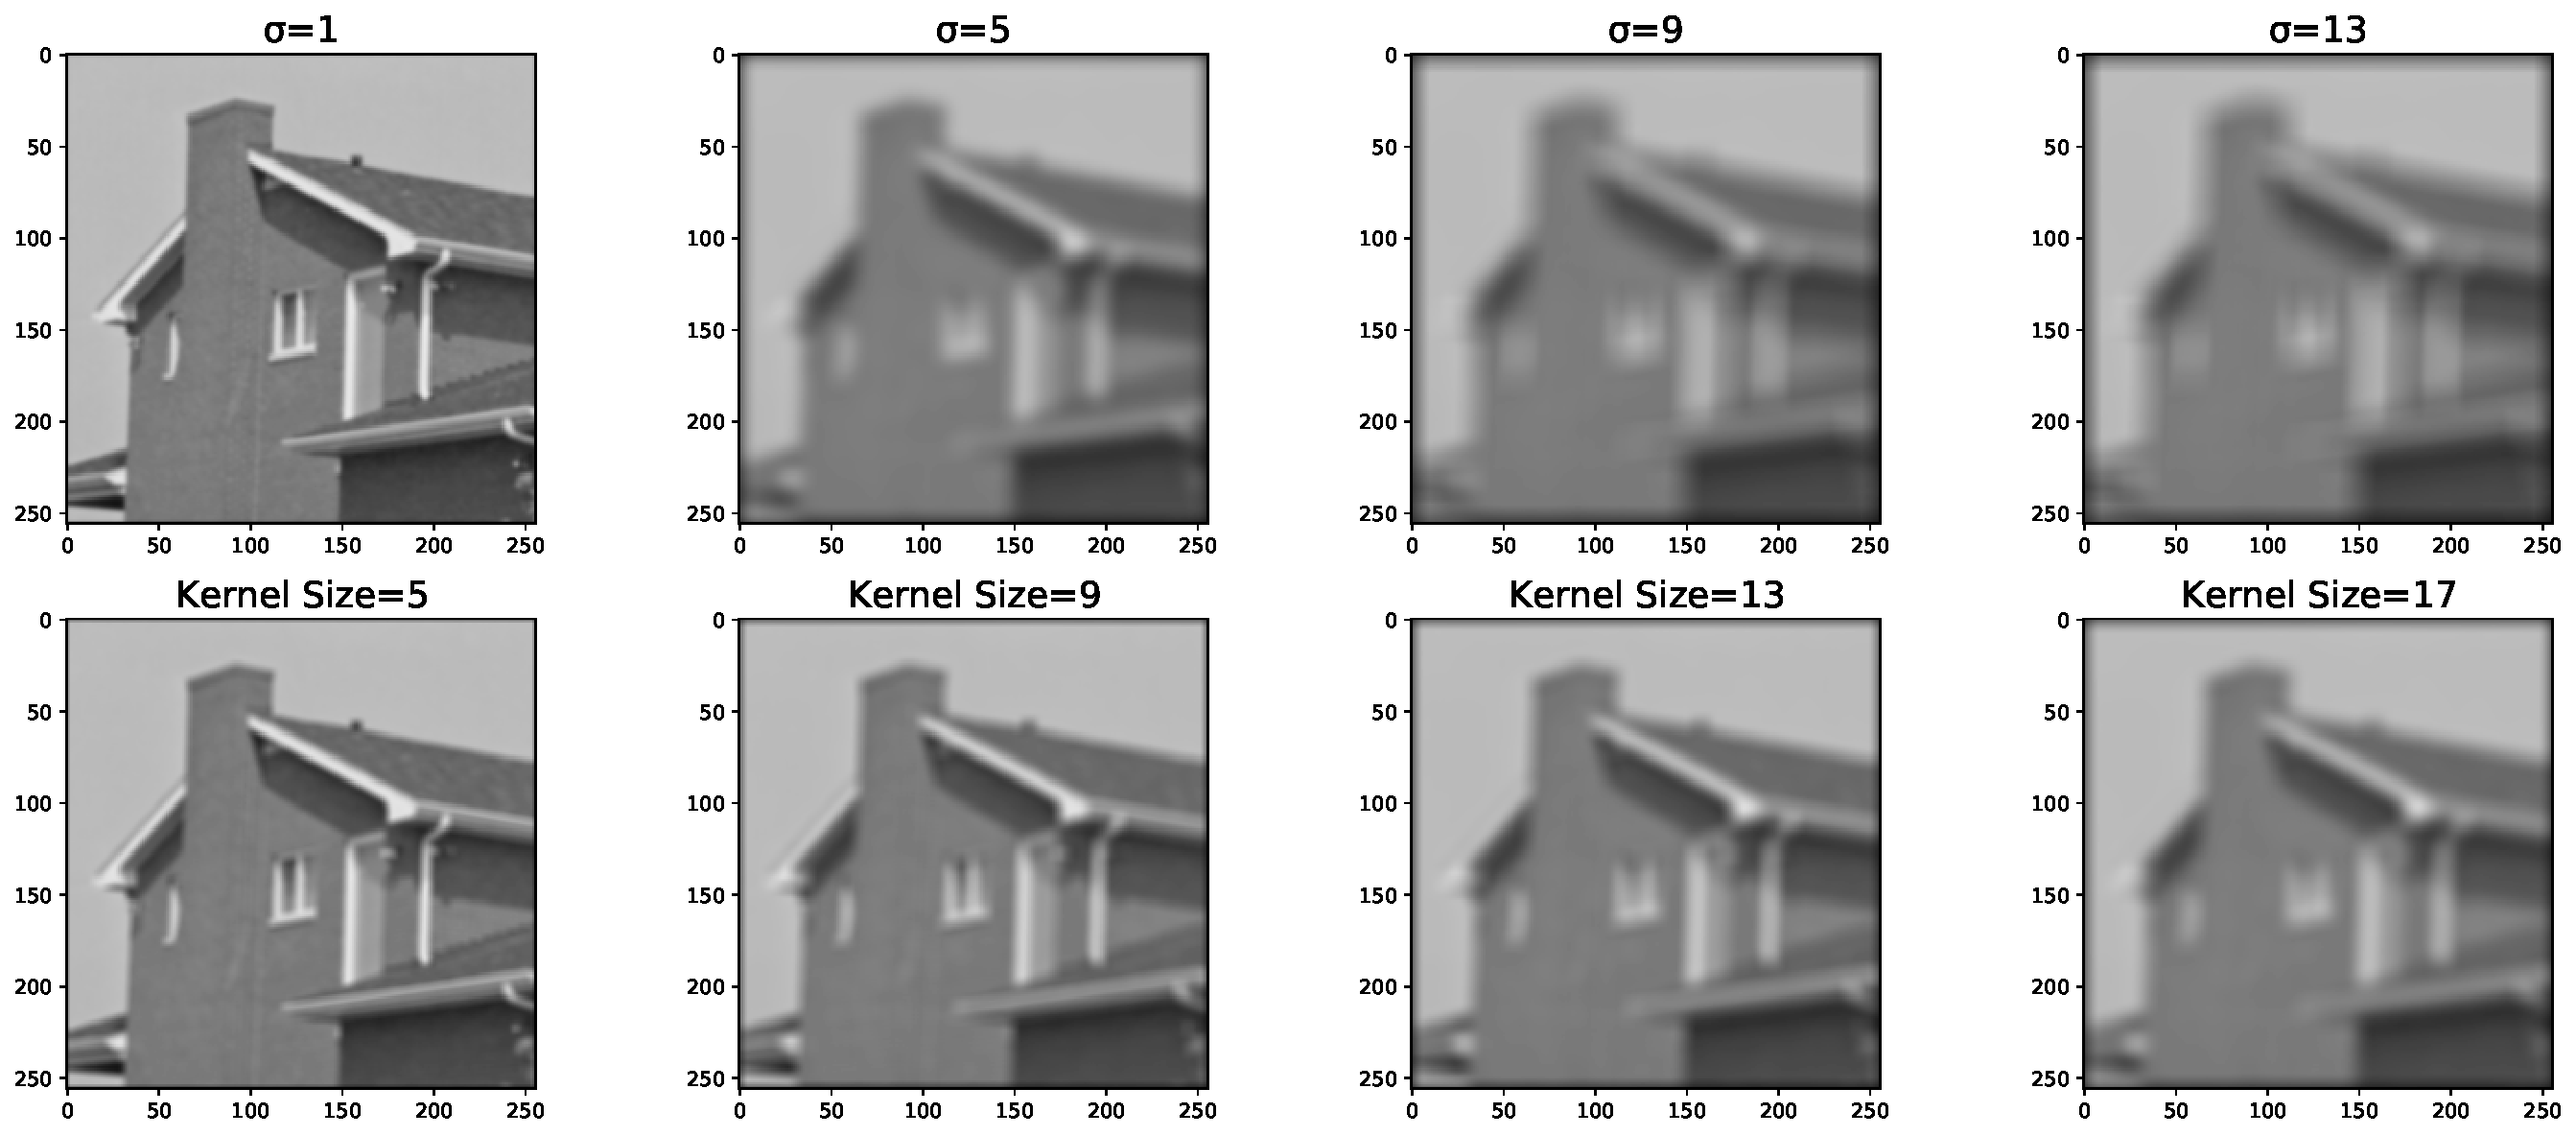
\includegraphics[width=1.0\linewidth]{Images/question_3_3.pdf}
\end{figure}
\end{solution}

\subsection{Blurring Justification \mypoints{2.0}}

Provide justification as to why the blurring effect increases with the kernel size and $\sigma$?


\begin{solution}
(i) Change of blurring effect of kernel size\\
Kernel size of a Gaussian kernel controls the number of pixel around the mean values that are taken into computation while applying the filter. A larger value of the kernel size implies a bigger filter, i.e. more pixel around the mean pixel contribute to the value of the current pixel leading to an blurrier image.

(ii) Blurring effect of $\sigma$\\
Variance $\sigma^2$ of a Gaussian kernel controls the spread of the output of the function around the mean value. A large value of $\sigma$ signifies a wider spread or more variance around the mean. Since a values father away from the mean position has a increased weightage the overall image is blurrier.

\end{solution}

\subsection{Median Filtering \mypoints{3.0}}
In this question you will be writing a Python function which performs median filtering given an input image and the kernel size. (See the Jupyter notebook.)

Make sure that your code is within the bounding box.
\begin{solution}
% \vspace{2cm} % remove this
% Paste your code within the block
\begin{minted}{python}
def median_filtering(image: np.array, kernel_size: int = None):
  pad_factor = int(kernel_size/2) #padding each side
  i_shape = image.shape #shape of the input image
  image = np.pad(image, ((pad_factor,pad_factor),(pad_factor,pad_factor)),
                 'constant') #padded image
  i_new_shape = image.shape #shape of the new image
  output = np.zeros(i_shape) #New convoluted image (all zeros)
  for i in range(i_new_shape[0] - kernel_size + 1):
    for j in range(i_new_shape[0] - kernel_size + 1):
      output[i][j] = np.median(image[i:i+kernel_size,j:j+kernel_size])

  return output
\end{minted}
\end{solution}

\subsection{Denoising \mypoints{1.0}}
(See the Jupyter notebook.)

Copy the saved image from the Jupyter notebook here.
\begin{solution}
% \vspace{2cm} % remove this
% Upload the image the Images folder in the project and then just un-comment the lines below.
\begin{figure}[H]
    \centering
    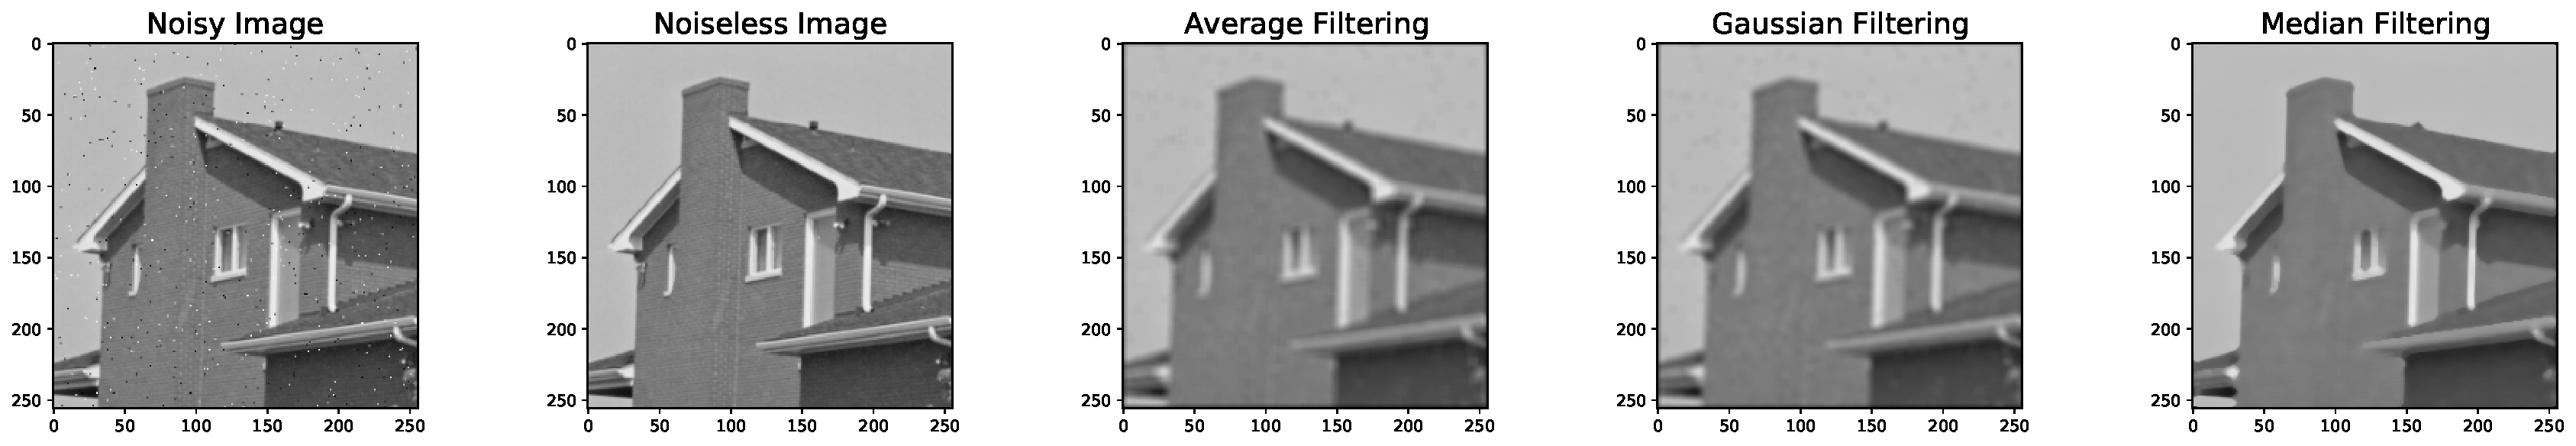
\includegraphics[width=1.0\linewidth]{Images/question_3_5.pdf}
\end{figure}
\end{solution}

\subsection{Best Filter \mypoints{2.0}}
In the previous part which filtering scheme performed the best? And why?
\begin{solution}
The median filtering scheme gives the best result amongst all other filters because it has clearest edge and minimal blurring outputting a sharper image.\\
This is also validated from the relative absolute distance. Median filter has the smallest value indicating maximum closeness to original image.\\

Average Filtering: 0.06525493187234264\\
Gaussian Filtering: 0.05995105367092967\\
Median Filtering: 0.03332913485508449\\
\end{solution}

\subsection{Preserving Edges \mypoints{2.0}}
Which of the 3 filtering methods preserves edges better? And why? Does this align with the previous part?
\begin{solution}
The median filter preserves the edge. 

This is because unlike other filters median filter does not act like a low pass filter. Noise is generally assumed to be an outlier and median filter finds the mid most element (in terms of pixel intensity) for a given kernel. Preserving the edges of the image and weeding out the noise.

This aligns with the previous answer.

\end{solution}

\newpage
\section{Image Gradients \mypoints{5.0}}
In this question you will be visualizing the edges in an image by using gradient filters. Gradients filters, as the name suggests, are used for obtaining the gradients (of the pixel intensity values with respect to the spatial location) of an image, which are useful for edge detection.

\subsection{Horizontal Gradient \mypoints{1.0}}
In this sub-part you will be designing a filter to compute the gradient along the horizontal direction.
(See the Jupyter notebook.) 

Make sure that your code is within the bounding box.
\begin{solution}
% \vspace{2cm} % remove this
% Paste your code within the block
\begin{minted}{python}
gradient_x = np.matmul(np.array([[1, 1, 1]]).transpose(),
                             np.array([[1, 0, -1]]))
\end{minted}
\end{solution}

\subsection{Vertical Gradient \mypoints{1.0}}
In this sub-part you will be designing a filter to compute the gradient along the vertical direction.
(See the Jupyter notebook.) 

Make sure that your code is within the bounding box.
\begin{solution}
% \vspace{2cm} % remove this
% Paste your code within the block
\begin{minted}{python}
gradient_y = np.matmul(np.array([[1, 0, -1]]).transpose(),
                             np.array([[1, 1, 1]]))
\end{minted}
\end{solution}

\subsection{Visualizing the gradients \mypoints{1.0}}
(See the Jupyter notebook.)

Copy the saved image from the Jupyter notebook here.
\begin{solution}
% \vspace{2cm} % remove this
% Upload the image the Images folder in the project and then just un-comment the lines below.
\begin{figure}[H]
    \centering
    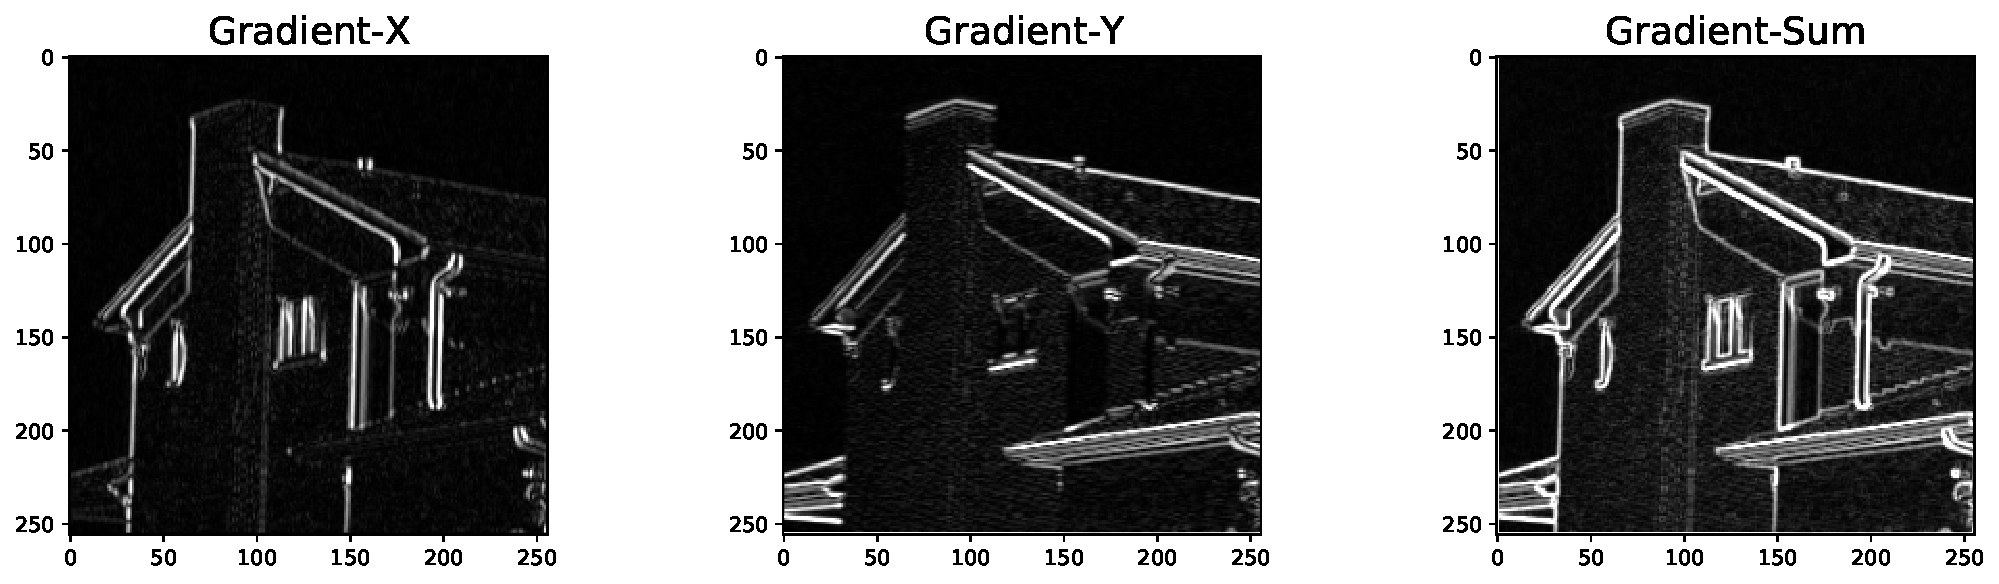
\includegraphics[width=1.0\linewidth]{Images/question_4_3.pdf}
\end{figure}
\end{solution}

\subsection{Gradient direction \mypoints{1.0}}
Using the results from the previous part how can you compute the gradient direction at each pixel in an image?

\begin{solution}
The gradient direction at each pixel in a image in calculated from the following formula:\\
$g[x,y] = \tan^{-1}(S_y/S_x)$\\
Where $S_y$ is the gradient in y direction and $S_x$ is the gradient in x direction at point (x,y).

\end{solution}

\subsection{Separable filter \mypoints{1.0}}
Is the gradient filter separable? If so write it as a product of 1D filters.

\begin{solution}
% \vspace{2cm} % remove this
yes,\\
$$H_x^P = \begin{bmatrix}
1\\
1\\
1\\
\end{bmatrix} 
\times
\begin{bmatrix}
1 & 0 & -1\\
\end{bmatrix}$$ \\

$$H_y^P = \begin{bmatrix}
1\\
0\\
-1\\
\end{bmatrix} 
\times
\begin{bmatrix}
1 & 1 & 1\\
\end{bmatrix}$$ \\
\end{solution}


\newpage
\section{Beyond Gaussian Filtering \mypoints{15.0}}
\label{Gaussian Filtering}
\subsection{Living life at the edge \mypoints{3.0}}\label{sssec:derivation}
The goal is to understand the weakness of Gaussian denoising/filtering, and come up with a better solution. In the lecture and the coding part of this assignment, you would have observed that Gaussian filtering does not preserve edges. Provide a brief justification.

[Hint: Think about the frequency domain interpretation of a Gaussian filter and edges.]
\begin{solution}
Gaussian filtering/denoising on a image has a blurring or smoothing effect due to its frequency response. It acts at a low pass filter that attenuates high spatial frequency components from a image. This helps in image denoising as noise are random outlier point in a image which causes high frequency change locally. On the other hand, edge in a images are regions of high frequency as there is rapid change in spatial properties just across the edge. While applying a Gaussian filter (low pass filter) the localization properties of the edge is not preserved.
\end{solution}

\subsection{How to preserve edges \mypoints{2.0}} \label{sssec:kernelshape}
Can you think of 2 factors which should be taken into account while designing filter weights, such that edges in the image are preserved? More precisely, consider a filter applied around pixel $p$ in the image. What 2 factors should determine the filter weight for a pixel at position $q$ in the filter window?
\begin{solution}
A filter should be such that the localization information of an image should be preserved.
Two factors to be taken in account for designing such a filter is:\\
(i) Distance between the pixel p and q , i.e. ($ \|p-q\|$)\\
(ii) Intensity difference between the pixel at p and q, i.e. ($ \|I_p-I_q\|$)
\end{solution}
    
\subsection{Deriving a new filter \mypoints{2.0}} \label{sssec:scenedepth}
For an image $I$, we can denote the output of Gaussian filter around pixel $p$ as $$ GF[I_p] = \sum_{q \in S} G_{\sigma}\big(\|p - q\|\big)I_{q}.$$

$I_p$ denotes the intensity value at pixel location $p$, $S$ is the set of pixels in the neighbourhood of pixel $p$. $G_{\sigma_p}$ is a 2D-Gaussian distribution function, which depends on $\|p - q\|$, i.e. the spatial distance between pixels $p$ and $q$. 
Now based on your intuition in the previous question, how would you modify the Gaussian filter to preserve edges? 

[Hint: Try writing the new filter as $$BF[I_p] = \sum_{q \in S} G_{\sigma}\big(\|p-q\|\big)f\big(I_{p}, I_{q}\big)I_q.$$ What is the structure of the function $f(I_{p}, I_{q})$? An example of structure is $f(I_{p}, I_{q}) = h(I_{p} \times I_{q})$ where $h(x)$ is a monotonically increasing function in $x$?]
\begin{solution}
$f(I_{p}, I_{q})$ can be a function that weigh outs /removes image pixels whose values differ drastically from the central pixel while denoising the images. This is a data dependent operation that measures the  similarity in intensity values to the middle pixels. Such a function can be the be Gaussian filter with mean around the central pixel.\\
$$f(I_{p}, I_{q}) = G_{\sigma} \big(\|I_{p}-I_{q}\|\big)$$

\end{solution}


\subsection{Complete Formula \mypoints{3.0}} \label{sssec:focallength}
Check if a 1D-Gaussian function satisfies the required properties for $f(.)$ in the previous part. Based on this, write the complete formula for the new filter $BF$.
\begin{solution}
Yes, a 1D Gaussian filter will satisfy the following criteria as it will softly reject pixels with higher intensity difference.\\
$$BF[I_p] = \sum_{q \in S} G_{\sigma_r}\big(\|p-q\|\big)G_{\sigma_d} \big(\|I_{p}-I_{q}\|\big)I_q.$$
\end{solution}
    
\subsection{Filtering \mypoints{3.0}}
In this question you will be writing a Python function for this new filtering method (See the Jupyter notebook.)

Make sure that your code is within the bounding box.
\begin{solution}
% Paste your code within the block
\begin{minted}{python}
def filtering_2(image: np.array, kernel: np.array = None, 
                sigma_int: float = None, norm_fac: float = None):

  k_shape = kernel.shape #shape of the kernel
  pad_factor = int(k_shape[0]/2) #padding each side
  i_shape = image.shape #shape of the input image
  image = np.pad(image, ((pad_factor,pad_factor),(pad_factor,pad_factor)), 
                 'constant') #padded image
  i_new_shape = image.shape #shape of the new image
  conv_matrix = np.zeros(i_shape) #New convoluted image (all zeros)

  for i in range(i_new_shape[0] - k_shape[0] + 1):
    for j in range(i_new_shape[0] - k_shape[0] + 1):
      image_sec = image[i:i+k_shape[0],j:j+k_shape[0]]
      d_guass = np.zeros(image_sec.shape)
      mxy = image_sec[size//2, size//2]
      c = 1 / (2*(sigma_int**2)*np.pi)
      # c = 1
      for idx, ixy in np.ndenumerate(image_sec):
        d_guass[idx] = c * np.exp(-((ixy - mxy)**2)/(2*(sigma_int**2)))

      conv_matrix[i][j] = \
      np.sum(np.multiply(np.multiply(d_guass,kernel),image_sec)) * norm_fac

  return conv_matrix

\end{minted}
\end{solution}

\subsection{Blurring while preserving edges \mypoints{1.0}}
Copy the saved image from the Jupyter notebook here.
\begin{solution}
% \vspace{2cm} % remove this
\begin{figure}[H]
    \centering
    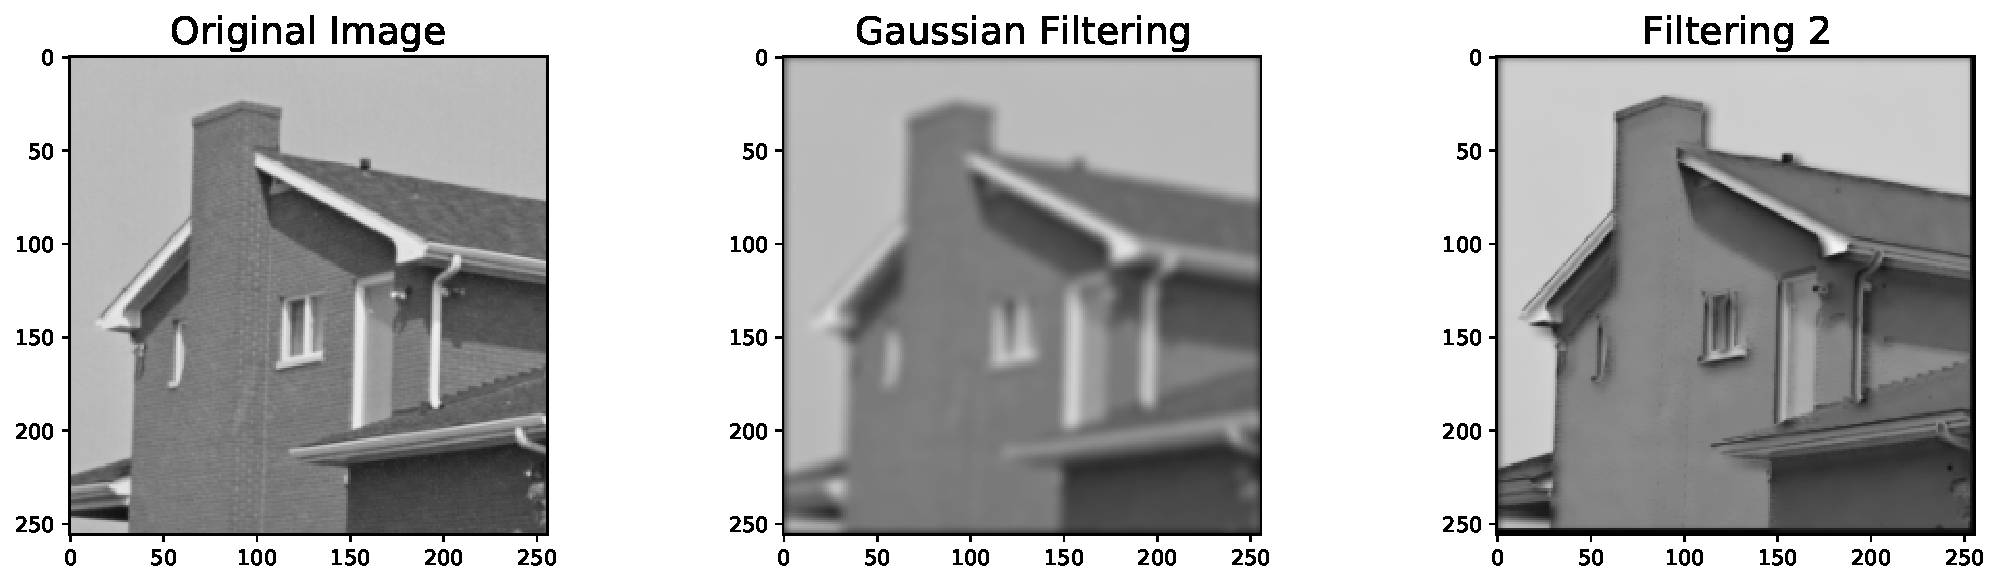
\includegraphics[width=1.0\linewidth]{Images/question_5_6.pdf}
\end{figure}
\end{solution}

\subsection{Cartoon Images \mypoints{1}} \label{sssec:focallength}
Natural images can be converted to their cartoonized versions using image processing techniques. A cartoonized image can generated from a real image by enhancing the edges, and flattening the intensity variations in the original image. What operations can be used to create such images?
[Hint: Try using the solutions to some of the problems covered in this homework.] 
\begin{figure}[H]
    \centering
    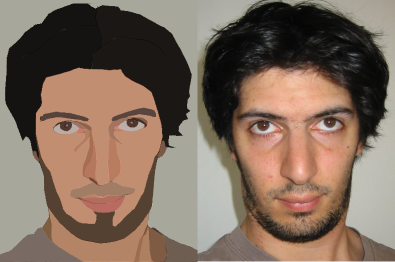
\includegraphics[width=0.5\linewidth]{Images/cartoon.png}
    \caption{(a) Cartoonized version (b) Natural Image}
\end{figure}
\begin{solution}
Cartooniztion can be achieved through the following sequence of operation:\\
(i) Bilateral Filtering : It will smoothen out the noise in the image while maintaining sharpness of the edges.\\
(ii) Median Filtering : It will remove outlier noise and further make the image intensity variation uniform.\\
(iii) Canny Edge Detection: It will be able to detect prominent edges in the images which can be used to enhance the edge pixels to give sharper boundaries. 
\end{solution}

\section{Interview Question (Bonus) \mypoints{10}}
Consider an $256 \times 256$ image which contains a square ($9 \times 9$) in its center. The pixels inside the square have intensity 255, while the remaining pixels are 0. What happens if you run a $9 \times 9$ median filter infinitely many times on the image? Justify your answer.

Assume that there is appropriate zero padding while performing median filtering so that the size of the filtered image is the same as the original image. 

\begin{solution}
The median filter works by returning the median element (in terms of pixel intensity) of all the pixels of the image overlapping with the kernel. While performing the median filtering over a binary image of the square, the filter will only return a value of 255 if at least 50\% of intensity values overlapping with the kernel have a value of 255. In case of a 9x9 kernel this value is at least 41. \textbf{When you apply the filter over the square image, the square will start diminishing from the outermost pixel (i.e. vertices) to the innermost pixel (i.e. center) after each iteration in a symmetric fashion till the square vanishes.} The inward trend is due to the fact the the vertex pixels have the least surrounding pixels with value 255 (i.e. 24) while the center pixel has the most (i.e 80).

% \begin{figure}[H]
%     \centering
%     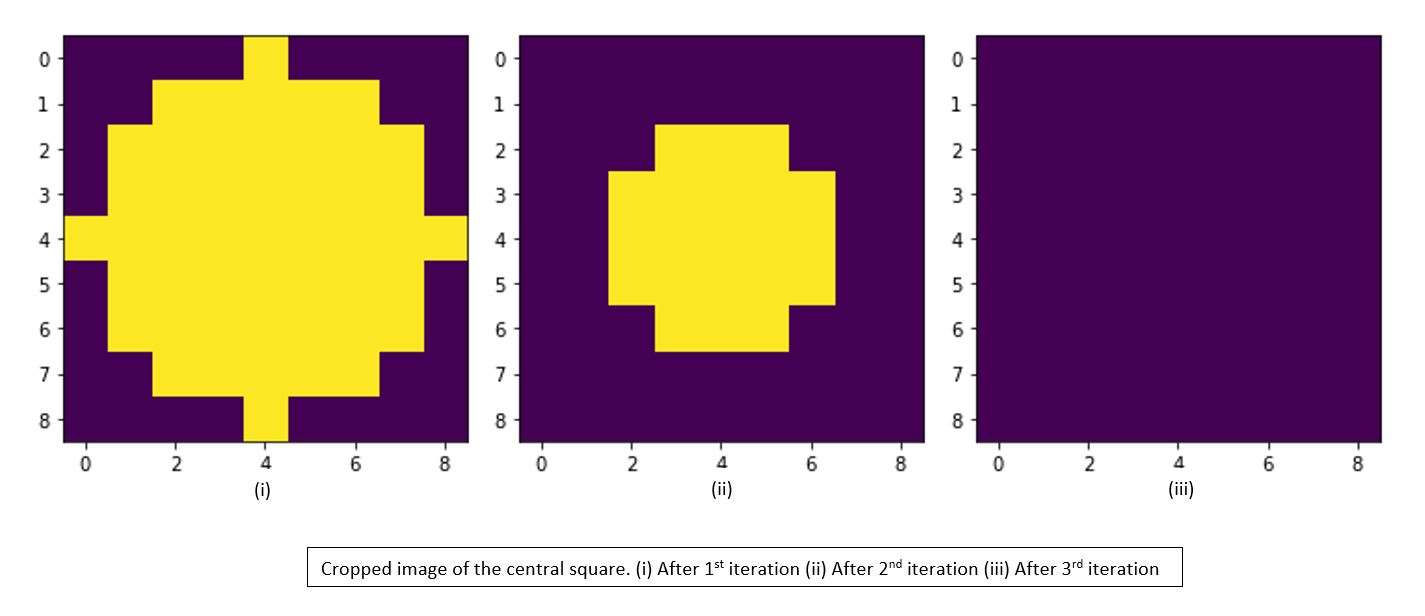
\includegraphics[width=1\linewidth]{Images/Capture.JPG}

% \end{figure}
\end{solution}

% \bibliographystyle{plain}
% \bibliography{bibliography.bib}


\end{document}